\section{Quantitative Evaluation}
\label{sec:results}

Table~\ref{tab:main_results} reports the final test-set metrics for both models. The exact values are generated automatically by \texttt{src/evaluate.py} and imported directly into the paper. Random Forest achieves the strongest Accuracy (0.8622), Precision (0.7812), and ROC-AUC (0.9141). In contrast, MLP achieves stronger Recall (0.6269) and a slightly better F1-score (0.6765), which was also the model-selection metric.

\IfFileExists{../outputs/tables/main_results_table.tex}{
    \input{../outputs/tables/main_results_table.tex}
}{
    \begin{table}[t]
    \centering
    \caption{Test-set classification metrics for the two compared models.}
    \label{tab:main_results}
    \begin{tabular}{lccccc}
    \toprule
    Model & Acc. & Prec. & Rec. & F1 & ROC-AUC \\
    \midrule
    Random Forest & TBD & TBD & TBD & TBD & TBD \\
    MLP & TBD & TBD & TBD & TBD & TBD \\
    \bottomrule
    \end{tabular}
    \end{table}
}

Table~\ref{tab:complexity_results} summarises the computational trade-offs. MLP is substantially more efficient: it trains in 7.92 seconds compared with 15.65 seconds for Random Forest, uses far less additional memory (1.28 MB vs.\ 175.66 MB), performs much faster inference per sample, and produces a dramatically smaller serialized model.

\IfFileExists{../outputs/tables/complexity_table.tex}{
    \input{../outputs/tables/complexity_table.tex}
}{
    \begin{table}[t]
    \centering
    \caption{Complexity and efficiency comparison on the held-out test set.}
    \label{tab:complexity_results}
    \begin{tabular}{lcccc}
    \toprule
    Model & Train(s) & Infer(ms) & Memory(MB) & Size(MB) \\
    \midrule
    Random Forest & TBD & TBD & TBD & TBD \\
    MLP & TBD & TBD & TBD & TBD \\
    \bottomrule
    \end{tabular}
    \end{table}
}

\begin{figure}[t]
    \centering
    \IfFileExists{../outputs/figures/roc_curve.pdf}{
        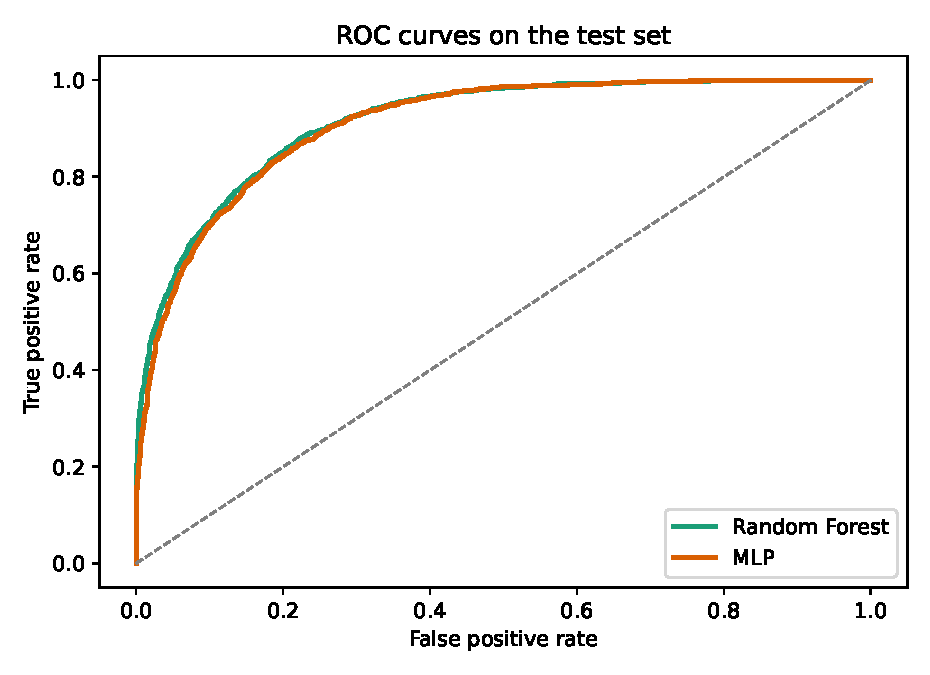
\includegraphics[width=\linewidth]{../outputs/figures/roc_curve.pdf}
    }{
        \fbox{\rule{0pt}{1.65in}\rule{0.95\linewidth}{0pt}}
    }
    \caption{ROC curves for the two models on the test split.}
    \label{fig:roc_curve}
\end{figure}

\begin{figure}[t]
    \centering
    \IfFileExists{../outputs/figures/rf_feature_importance.pdf}{
        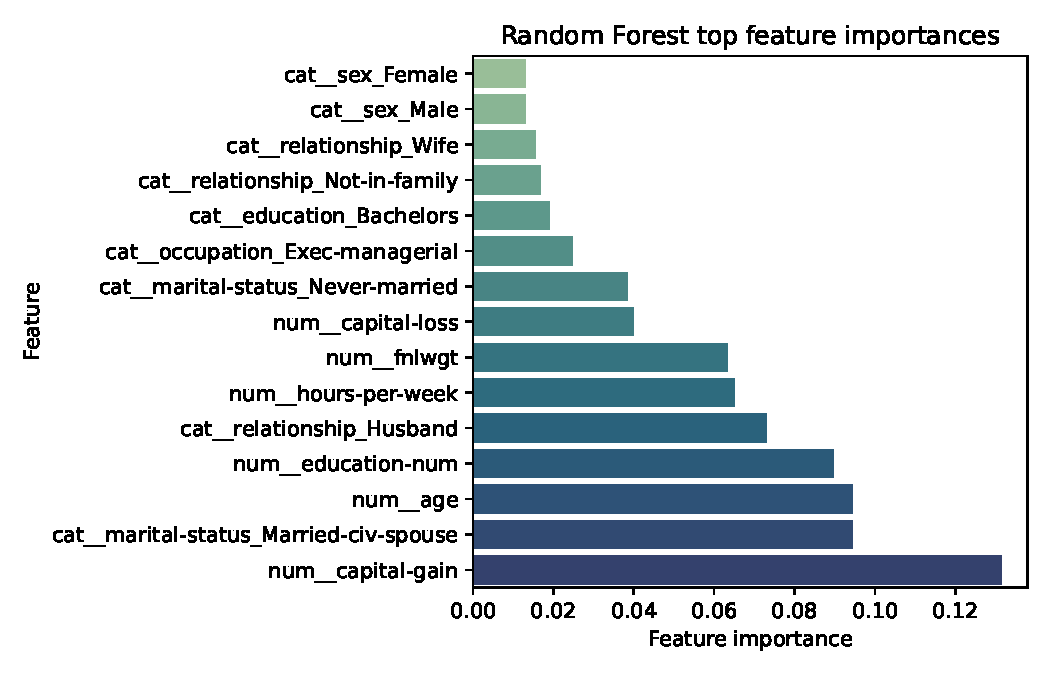
\includegraphics[width=\linewidth]{../outputs/figures/rf_feature_importance.pdf}
    }{
        \fbox{\rule{0pt}{1.65in}\rule{0.95\linewidth}{0pt}}
    }
    \caption{Random Forest feature importance visualisation.}
    \label{fig:rf_importance}
\end{figure}

\paragraph{Discussion.}
The comparison shows that neither model dominates every metric, so the headline result is a trade-off rather than a simple winner. Relative to MLP, Random Forest improves Precision by 4.66 percentage points and ROC-AUC by 0.54 points, but loses 3.82 points of Recall and 0.51 points of F1. In confusion-matrix terms, the MLP identifies 67 additional true high-income cases on the test set, but it also introduces 108 more false positives. This is a useful difference to report because it explains how two models with similar overall scores can behave differently in practice.

The ROC curves in Figure~\ref{fig:roc_curve} show that both models separate the classes well overall, with only a modest gap between them. The main difference is therefore not raw separability, but operating behaviour at the default decision threshold. Random Forest is the more conservative classifier: when it predicts income above \$50K, it is more often correct, but it also leaves more positive cases undiscovered. The MLP behaves in the opposite way, sacrificing some precision to recover more of the minority class.

Figure~\ref{fig:rf_importance} also makes the result easier to interpret. The most influential Random Forest features are capital gain, marital-status indicators, age, education-num, relationship, and hours-per-week. These variables are plausible for the Adult task and align with the intuition that income is associated with accumulated earnings signals, life stage, and labour-market position. At the same time, the importance ranking should not be read as causal evidence; it only indicates which variables helped this model partition the dataset most effectively.

Taken together, the results suggest that MLP is the better default choice when storage, memory use, and balanced retrieval matter most, especially because its F1-score is the strongest while its computational footprint is tiny. Random Forest remains attractive when the user values conservative positive predictions, slightly stronger discrimination, and easier post-hoc explanation of what drove the model's decisions.
